\documentclass{report}
\usepackage[francais]{babel}
\usepackage[utf8]{inputenc}
\usepackage[T1]{fontenc}
\usepackage{float}
\usepackage{amssymb}
\usepackage{stmaryrd}

\usepackage{graphicx}
\usepackage{subfig}

\makeatletter
\newcommand{\Spvek}[2][r]{%
  \gdef\@VORNE{1}
  \left(\hskip-\arraycolsep%
    \begin{array}{#1}\vekSp@lten{#2}\end{array}%
  \hskip-\arraycolsep\right)}

\def\vekSp@lten#1{\xvekSp@lten#1;vekL@stLine;}
\def\vekL@stLine{vekL@stLine}
\def\xvekSp@lten#1;{\def\temp{#1}%
  \ifx\temp\vekL@stLine
  \else
    \ifnum\@VORNE=1\gdef\@VORNE{0}
    \else\@arraycr\fi%
    #1%
    \expandafter\xvekSp@lten
  \fi}
\makeatother

\newcommand{\HRule}{\rule{\linewidth}{0.5mm}}
\bibliographystyle{unsrt}
\begin{document}

\begin{titlepage}

\begin{center}

\textsc{\LARGE \'Etat de l'art}\\[1.5cm]

\textsc{\Large EPITA}\\[0.5cm]

\HRule \\[0.4cm]
{ \huge \bfseries MLEA - Empreintes digitales}\\[0.4cm]

\HRule \\[1.5cm]

\large
\emph{Auteurs:}\\
Thomas \textsc{Badie}\\
Victor \textsc{Lenoir}\\
David \textsc{Moreira}\\
Pierre \textsc{Parutto}\\

\vfill

% Bottom of the page
{\large \today}

\end{center}

\end{titlepage}
%\maketitle
\newpage
\tableofcontents
\newpage

\chapter{Introduction}
La reconnaissance d'empreintes digitales consiste en une
reconnaissance d'un motif (empreinte sur le doigt) permettant
d'identifier le possesseur de cette empreinte. Il y a deux types
d'applications utilisant la reconnaissance d'empreintes :

\begin{description}
\item[Vérification] Une personne décline son identité et on vérifie
  que c'est vrai en comparant l'empreinte sur le doigt avec celle dans
  la base et on répond oui ou non ;
\item[Identification] On n'a aucun indice à l'avance sur l'identité du
  possesseur de l'empreinte. Il faut donc comparer l'image à toutes
  celles de la base.
\end{description}

La phase d'acquisition, généralement commune aux deux types
d'applications, correspond à l'enregistrement de l'empreinte dans la
base de donnée. Elle est généralement suivie par une algorithme de
validation de la qualité de l'enregistrement comme le montre la Figure
\ref{fig:schema-bloc-acq}.

\begin{figure}[H]
\centering
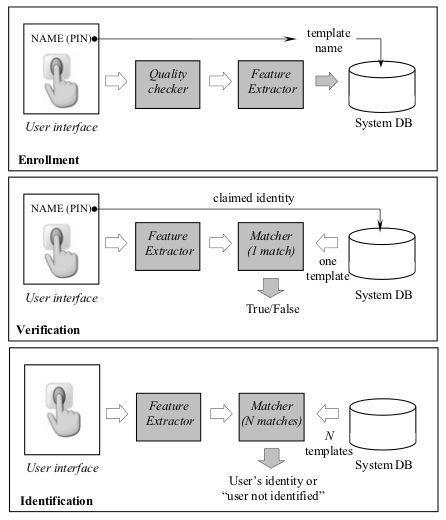
\includegraphics[scale=0.8]{three_way.png}
\caption{Schéma bloc de l'acquisition, de la vérification et de
  l'identification.}
\label{fig:schema-bloc-acq}
\end{figure}

Comme on peut le voir sur la Figure, l'image est ensuite transformée
en un modèle (\emph{template} en anglais) grâce à un extracteur de
caractéristiques (\emph{feature extractor} en anglais).

Dans le cas de la vérification, l'utilisateur entre son identifiant et
donne son empreinte. Celle-ci est transformée en un modèle compact.
On extrait le modèle lui correspondant dans la base de donnée, et un
comparateur est chargé de prendre la décision \og oui / non \fg.

Dans le cas de l'identification, c'est différent car il n'y a aucun
identifiant qui est donné et ce n'est plus un simple écart entre deux
modèles à calculer, mais un écart avec toutes les données de la base.
Les résultats possibles sont l'identité du possesseur des empreintes,
ou \og utilisateur non identifié \fg.

Il y a différentes parties distinctes, et dans un premier temps, nous
allons traiter des problèmes liés à ce type de biométrie. Dans un
second temps, nous allons traiter deux méthodes permettant la
vérification ou l'identification d'individu. La première de ces
méthodes et la méthode basé sur la corrélation entre deux empreintes
digitales. La seconde méthode se base sur les défauts que peuvent
présenter les empreintes digitales.


%%% Local Variables:
%%% mode: latex
%%% TeX-master: "../mlea"
%%% End:


\section{Problèmes liés à la biométrie}

Il y a divers problèmes liés à cette biométrie, notamment lors de
l'acquisition. Il y a principalement deux moyens d'effectuer ce
processus \emph{off-line}, c'est à dire la méthode ancestrale avec de
l'encre sur le doigt et apposé sur du papier, et \emph{live} qui
correspond à utiliser un scanner numérique. Pour assurer une
compatibilité entre ses deux méthodes d'acquisition, le ``US Criminal
Justice Information Services'' a présenté un ensemble de
spécifications pour fixer la qualité et le format des images (voir
annexes F et G de \cite{nla.cat-vn4185009}).

Bien que la méthode à l'encre ait commencé à être utilisé il y a très
longtemps (plus d'une trentaine d'année) elle est toujours utilisée
dans des applications à caractères légales. Les bases de données des
agences américaines de sécurités contiennent des données ayant été
acquises par les deux méthodes, ce qui signifie que les algorithmes
travaillant sur ces bases doivent être capables de les traiter
indépendemment.

Un des avantages d'utiliser l'acquisition avec l'encre est que l'on
peut enregistrer tout le doigt en effectuant un mouvement rotatif en
partant avec son doigt perpendiculaire d'un côté pour aller à
perpendiculaire de l'autre, ce qui n'est pas possible avec un scanner
numérique.

En contrepartie, il est possible, en fonction de comment est placée
l'encre sur le doigt, de laisser des zones de vide ou alors trop
pleine.

Du côté des acquisitions numériques, la plupart des appareils peuvent
se classer dans trois catégories différentes :

\begin{description}
\item[Optiques] le plus vieux et le plus utilisé des techniques
  d'acquisitions actuelles. Cette méthode fonctionne avec un prisme en
  verre. L'utilisateur doit mettre son doigt en haut de ce prisme est
  l'acquisition se fait ainsi.

  Ce type d'appareil a l'avantage de faire des images de bonnes
  qualités et d'avoir une grande surface du doigt enregistrée. Par
  contre, on ne peut pas miniaturiser cet appareil ;
\item[Ultrasons] il s'agit d'envoyer des ultrasons sur le doigt et de
  récupérer l'écho. Il est ainsi possible de dessiner la structure de
  l'empreinte digitale. Les images sont de bonne qualités, mais le
  système est onéreux ;
\item[Semi conducteurs] il y a quatre principales méthodes :
  thermique, capacitive, par champs électrique et piezoélectrique.  Il
  s'agit de toucher une carte en silice où chaque pixel est un petit
  capteur.
\end{description}

À présent que nous avons présenté les différentes manières de faire
l'acquisition, il nous faut à présent introduire quelques problèmes
communs à toutes les acquisitions. Il existe des variations en
fonction de l'état du doigt au moment de l'acquisition. Si celui-ci
est sec ou humide, l'image finale est différente.

Il existe aussi des problèmes de translation, de rotation ainsi que
des problèmes d'élasticité du doigt.


%%% Local Variables:
%%% mode: latex
%%% TeX-master: "../mlea"
%%% End:


\chapter{Correlation-based}
\chapter{Minuatiae Based}

La seconde méthode que nous allons traiter dans cet état de l'art est
la méthode basé sur l'extraction des minutia (ou minutiaes) sur les
empreintes digitales. Chaque empreinte comporte un certain nombre de
défaut, appelés minutiaes. Ces défauts sont unique pour chaque
individu. Cependant, il important de remarquer que l'on a une chance
sur dix milliards d'avoir des minutia qui peuvent être assez
ressemblant pour être confondues. Les minutia sont des défauts de
l'empreinte digitales qui sont définie dès la naissance et sont
inchangeable durant la vie entière de l'individu.

Pour effectuer cette technique, il nous faut d'abord extraire un
maximum de ces défauts pour que la méthode puisse fonctionner d'une
façon optimale. Dans la seconde partie nous traiterons la méthode
permettant de valider si deux empreintes appartient bien au même
individu et également au même doigt.

Selon la législation française, un individu peut être reconnut avec
seulement 12 minutiaes. Une empreinte digitale comporte en moyenne 100
de ces défauts et les méthodes communes travaillent sur environ 60\%
des minutiaes présent sur une empreinte digitale. Ainsi, selon la
législation française il est facile de faire correspondre deux
empreintes digitales.


\section{Détection des Minutiaes}

Les minutiaes sont classés en divers types selon leurs spécifications
et leurs formes géométrique. Ces défauts ont été classés en cinq
grands type par l'Ansi (pour American National Standards
Institute). Les trois types de minutiaes principaux sont la
terminaison, le branchement et l'intersection. Les autres types de
minutiaes sont en générales pas détecter car souvent confondues avec
des erreurs de l'acquisition de l'empreinte ou un pré-traitement non
favorable à leurs détection. Il faut cependant remarquer que la non
détection de ces minutiaes n'est pas discriminatoire pour le bon
fonctionnement de la comparaison de deux empreintes digitales. En
effet, si on ne considère que les cinq grands types de minutiaes de
l'Ansi, on arrive à une moyenne de 60 minutiaes par empreintes. Ce
nombre est donc suffisant pour identifier une personne de façon légale
en France.

La méthode la plus fiable et donc également la plus utilisé est le
parcours des lignes présentes sur les empreintes digitales. Afin
d'utiliser cette méthode il nous faut pré-traiter l'image afin de
suivre ces lignes.

Il existe deux méthode principales. La première est d'utiliser
l'empreinte digitale en niveau de gris avec les zones foncés étant les
lignes des empreintes digitales. Il faut donc détecter les lignes et
les suivre. Ainsi on peut détecter les terminaisons et les
bifurcations facile. Une méthode existe en utilisant le gradient de
l'image. La méthode reste sensiblement la même. Pour pouvoir suivre
les lignes on cherche dans une fenêtre centré en un point et ayant
comme dimension la distance locale entre deux lignes de
l'empreinte. On est donc obligé de calculer localement la distance
minimale entre deux lignes et  de chercher la direction de la ligne
que l'on parcourt.

\section{Épuration des minutiaes}

Lorsqu'on fait l'acquisition d'un empreinte digitale, il apparaît que
les lignes qui sont proches du bords de l'image sont coupé. On va donc
avoir des terminaisons qui vont être détecté à tort sur ces parties de
l'image. La solution pour ne plus avoir ce problème est de pas
considérer tous les minutiaes situées sur le bord de l'empreinte
digitale. De plus, on ignore tous les minutiaes et pas seulement les
terminaisons : cette parties de l'image produit beaucoup trop de faux
positif pour chercher à savoir si la minutiae en est une.

Le deuxième problème majeur est le regroupement de minutiaes.



\section{Comparaison des minutiaes}

Dans cette étape, on considère en entré deux ensembles: $p =
\{x_{i}^{p}, y_{i}^{p}, \theta_{i}^{p}\}, i \in \llbracket 1, M
\rrbracket$ et $q = \{x_{j}^{q}, y_{j}^{q}, \theta_{j}^{q}\}, j \in
\llbracket 1, N \rrbracket$ qui représentent les minutia extraites de
chacune des images à comparer. La comparaison entre les deux
empreintes digitales se ramène ainsi à compter le nombre de paires de
minutia identiques dans les deux ensembles et à comparer cette valeur
à un certain seuil. Cette comparaison se fait en deux étapes:

\begin{enumerate}
\item Trouver un alignement optimal;
\item Calculer la similarité.
\end{enumerate}

Pour chacune des ces étapes il existe plusieurs méthodes. Celle
présentée ci-dessous est tirée du cours~\cite{finger.00.jain} et les
illustration sont celles présentes dedans.

\subsection{Alignement}

Le problème d'alignement entre deux ensembles de minutia est
compliqué car on ne sait pas à l'avance la correspondance entre les
minutia des deux ensembles. De plus à cause des déformations dues au
bruit ajouté par les capteurs lors de l'acquisition des empreintes, il
est impossible de trouver un alignement exact. De ce fait l'alignement
entre les deux ensembles se fait en appliquant des déformations à l'un
jusqu'à minimiser la distance entre les deux ensembles. Ces
déformations sont de deux types: translations et rotations.\\
%% FIXME: @Pierre:Il y a aussi l'élasticité de la peau qui rentre en jeux.
Plus précisément, le repère pour l'alignement sont les crêtes
représentées par des signaux en 1-dimension. L'algorithme d'alignement
prend en entré deux ensembles de crêtes venant de chacune des images:
$R_p$ et $R_q$ et se déroule comme suit:

\begin{enumerate}
\item Prendre une paire de crêtes: $c \in R_p$ et $c' \in R_q$ et les
  comparer en utilisant la formule:
$$S = \frac{\sum\limits_{i=0}^L c_i c'_i}{\sqrt{\sum\limits_{i=0}^{L} c_{i}^2 c_{i}^{'2} }}$$
Avec:
\begin{itemize}
\item $L$: la taille de la plus petite crête,
\item $c_i$: la distance du point $i$ de la crête $c$ à l'axe des abscisses,
\item $c'_i$: la distance du point $i$ de la crête $c'$ à l'axe des abscisses ;
\end{itemize}
\item Si $S > seuil$ alors l'alignement est terminé ;
\item Sinon:
  \begin{itemize}
  \item Calculer le vecteur de translation:
    $$\Spvek{\Delta x \\ \Delta y} =  \Spvek{x_p \\ y_p} - \Spvek{x_q \\ y_q}$$
  \item Puis le vecteur de rotation:
    $$\Delta \theta  = \frac{1}{L} \sum\limits_{i = 0}^L (\varphi_i - \psi_i)$$
    avec $\varphi_i$ et $\psi_i$ les angles radiaux entre le $i^e$
    point et la minutiae de référence,
  \item Enfin appliquer la transformation suivante sur la minutiae :
    $$\Spvek{x_i \\  y_i \\ \theta_i} = \Spvek{\Delta x \\ \Delta y \\ \Delta \theta} +
    \left (
      \begin{array}{ccc}
        cos \Delta \theta & sin \Delta \theta & 0\\
        sin \Delta \theta & -cos \Delta \theta & 0\\
        0 & 0 & 1
      \end{array}
    \right )
    \Spvek{x_i - x_p \\ y_i - y_p \\ \theta_i - \theta_p}$$
  \end{itemize}
\item Recommencer à l'étape 1 avec une nouvelle paire de crêtes.
\end{enumerate}

Une fois que cette étape d'alignement est finie, l'alignement entre
les deux images est optimale et le calcul de similarité peut être
effectué.

\subsection{Calcul de similarité}

Une méthode pour calculer la similarité entre deux ensemble de
minutia consiste à les considérer comme des chaînes de caractères et
appliquer un algorithme de calcul de distance d'édition sur les deux
chaînes.\\

La conversion des ensembles de minutia en chaînes de caractères se
fait de la manière suivante : les coordonnées sont converties en
coordonnées polaires en fonction d'une minutiae de référence
choisie. Puis concaténer le résultat pour chaque minutiae par ordre
croissant d'angle radial :
$$P_p = \{(r_{1}^p, e_{i}^p, \theta_{1}^p), \ldots, (r_{M}^p, e_{M}^p, \theta_{M}^p)\}$$
$$Q_p = \{(r_{1}^q, e_{i}^q, \theta_{1}^q), \ldots, (r_{N}^q, e_{N}^q, \theta_{N}^q)\}$$

où $P$ et $Q$ sont donc deux chaînes de caractères.\\
% FIXME: @Pierre : Tu ne veux pas dire $P_p$ et $Q_p$ ?
La distance d'édition se calcule en utilisant un algorithme similaire
à celui de Levenshtein utilisant la programmation dynamique pour
remplir la matrice $C$ :
% FIXME: @Pierre : Pourquoi tu parles de programmation dynamique ? Si
% tu as une raison pourquoi parler de matrice (on utilises seulement un vecteur ?)
$$C(m,n) = \left \{
\begin{array}{ll}
  0 & \mbox{ si } m = 0 \land n = 0\\
  min \left \{
      \begin{array}{l}
        C(m - 1, n) + \Omega\\
        C(m, n - 1) + \Omega\\
        C(m - 1, n - 1) + w(m, n)
      \end{array}  \right . & \mbox {sinon }
\end{array} \right .
$$

Avec:

\begin{itemize}
\item $m \in \llbracket 0, M \rrbracket$ et $n \in \llbracket 0, N \rrbracket$
\item $w(m,n) = \left \{
    \begin{array}{ll}
      \alpha \mid r_{m}^p - r_{n}^q \mid + \beta \Delta e + \gamma \Delta \theta & \mbox { si } \mid r_{m}^p - r_{n}^q \mid < \delta \land \Delta e < \epsilon \land \Delta \theta < \rho \\
      \Omega & \mbox{ sinon}
    \end{array} \right .$
\item $\Delta e = \left \{
    \begin{array}{ll}
      a & \mbox { si } (a = (e_{m}^p - e_{n}^q + 360) \mbox{ mod } 360) < 180\\
      a - 180 & \mbox { sinon }
    \end{array} \right . $
\item $\Delta \theta = \left \{
    \begin{array}{ll}
      a & \mbox { si } (a = (\theta_{m}^p - \theta_{n}^q + 360) \mbox{ mod } 360) < 180\\
      a - 180 & \mbox { sinon }
    \end{array} \right . $
\end{itemize}

Et la signification des constantes est la suivante :
\begin{itemize}
\item $\alpha$, $\beta$, $\gamma$ sont les poids associés au rayon,
  angle radial et orientation ;
\item $\delta$, $\epsilon$, $\rho$ représentent la bounding-box ;
\item $\Omega$ est une pénalité de différence fixé.
\end{itemize}

L'image~\ref{fig:match} présente un exemple graphique des résultats de
la méthode présenté.

\begin{figure}
  \centering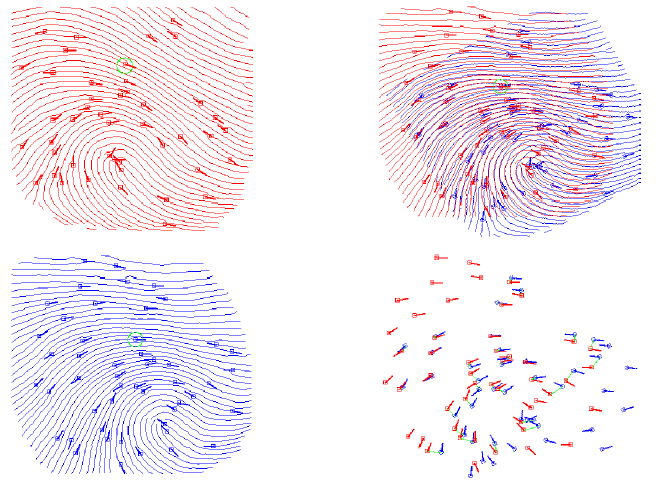
\includegraphics[scale=.4]{figres.png}
  \caption{Un exemple d'utilisation de la méthode.}
  \label{fig:match}
\end{figure}

La distance d'édition ainsi calculée est appelée $M_{pq}$ et permet de
calculer le score de similarité $S$ via la formule :
$$S = \frac{100 (M_{pq})^2}{MN}$$

La présentation donnée de l'algorithme possède quelque limitations, en
effet il tolère bien les transformations inexactes et/ou non linéaires
mais ne peut pas les compenser. Pour cela il faudrait utiliser la
méthode des bounding-box adaptatives permettant une meilleur
correspondance entre les bounding box.\\

La complexité de l'algorithme de Levenshtein est avec l'implémentation
classique en $O(NM)$ avec $N$ et $M$ les tailles des deux
chaînes. Cependant un fort surcoût apparaît à cause du calcul des
différents poids et notamment de w. L'image~\ref{fig:recap} présente un schéma
récapitulatif de la méthode.
% FIXME: @Pierre : L'algorithme de Levenshtein est toujours en
% O(MN). Seul la consommation mémoir peut être réduite.
\begin{figure}
  \hspace{-10em}
  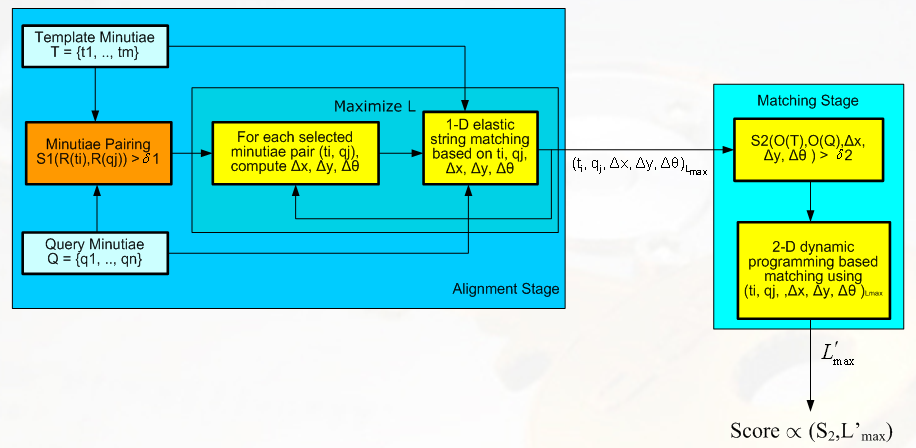
\includegraphics[scale=.6]{figrecap.png}
  \caption{Graphique récapitulant les grandes étapes de la méthode.}
  \label{fig:recap}
\end{figure}

\subsection{Performances}
\label{sec:performances}

En ce qui est des performances, cette méthode a été testé par les
auteurs de la présentation sur la base de données FVC2002 1. Cette
base contient 100 utilisateur avec chacun 8 empreintes.

Les résultats de la méthode sur cette base sont les suivants:
\begin{itemize}
\item Taux de fausses alarmes (FAR) : 0.1\%
\item Taux de vrai acceptation (GAR) : 97.6\%
\item Taux à erreurs égales (EER) : 1.65\%
\item Taux de fausse acceptation (FRR) : 4\%
\end{itemize}

De plus les courbes présentées dans l'image~\ref{fig:res} montrent
deux autres indicateurs. À titre de comparaison, l'algorithme donnant
les meilleur résultats sur cette base de donnée est PA15 et ses scores
sont les suivants:

\begin{itemize}
\item FAR : 0.11%
\item GAR : 100%
\item EER : 0.1%
\item FRR : 0%
\end{itemize}

On se rend donc compte que cette méthode donne des résultats très
satisfaisant et est proche de la meilleur méthode. Un paramètre que
nous n'avons pas réussi à trouver est le temps que met la méthodes
pour donner un résultat donc nous ne pouvons pas comparer ce critère.

\begin{figure}
  \centering\subfloat[Distribution des similaritées]{\hspace{-10em}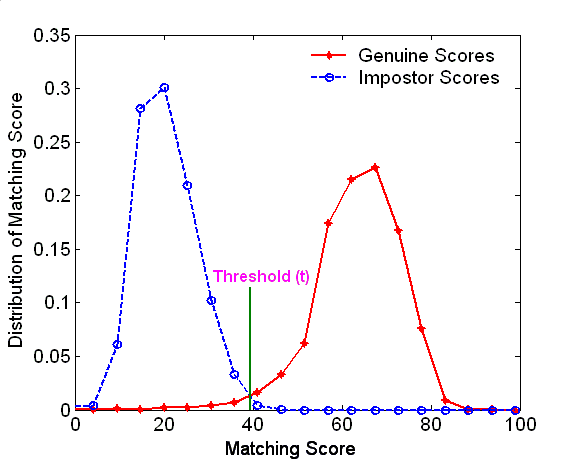
\includegraphics[scale=.5]{matchscore.png}}
  \centering\subfloat[Courbe ROC]{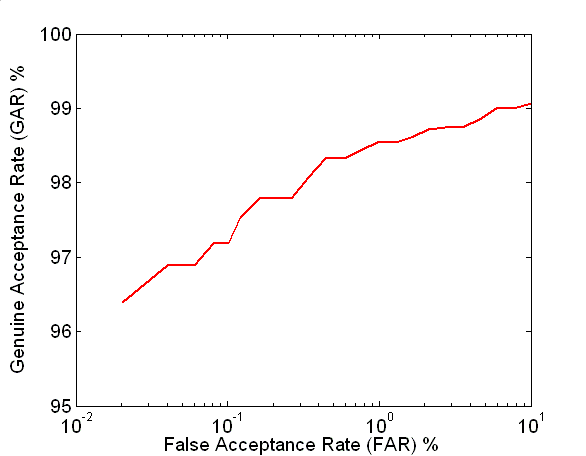
\includegraphics[scale=.5]{roccurve.png}}
  \caption{Deux autres indicateurs}
  \label{fig:res}
\end{figure}


\chapter{Conclusion}

\documentclass{report}
\usepackage[francais]{babel}
\usepackage[utf8]{inputenc}
\usepackage[T1]{fontenc}

\usepackage{amssymb}
\usepackage{stmaryrd}

\usepackage{graphicx}
\usepackage{subfig}

\makeatletter
\newcommand{\Spvek}[2][r]{%
  \gdef\@VORNE{1}
  \left(\hskip-\arraycolsep%
    \begin{array}{#1}\vekSp@lten{#2}\end{array}%
  \hskip-\arraycolsep\right)}

\def\vekSp@lten#1{\xvekSp@lten#1;vekL@stLine;}
\def\vekL@stLine{vekL@stLine}
\def\xvekSp@lten#1;{\def\temp{#1}%
  \ifx\temp\vekL@stLine
  \else
    \ifnum\@VORNE=1\gdef\@VORNE{0}
    \else\@arraycr\fi%
    #1%
    \expandafter\xvekSp@lten
  \fi}
\makeatother

\newcommand{\HRule}{\rule{\linewidth}{0.5mm}}
\bibliographystyle{unsrt}
\begin{document}

\begin{titlepage}

\begin{center}

\textsc{\LARGE \'Etat de l'art}\\[1.5cm]

\textsc{\Large EPITA}\\[0.5cm]

\HRule \\[0.4cm]
{ \huge \bfseries MLEA - Empreintes digitales}\\[0.4cm]

\HRule \\[1.5cm]

\large
\emph{Auteurs:}\\
Thomas \textsc{Badie}\\
Victor \textsc{Lenoir}\\
David \textsc{Moreira}\\
Pierre \textsc{Parutto}\\

\vfill

% Bottom of the page
{\large \today}

\end{center}

\end{titlepage}
%\maketitle
\newpage
\tableofcontents
\newpage

\chapter{Introduction}
La reconnaissance d'empreintes digitales consiste en une
reconnaissance d'un motif (empreinte sur le doigt) permettant
d'identifier le possesseur de cette empreinte. Il y a deux types
d'applications utilisant la reconnaissance d'empreintes :

\begin{description}
\item[Vérification] Une personne décline son identité et on vérifie
  que c'est vrai en comparant l'empreinte sur le doigt avec celle dans
  la base et on répond oui ou non ;
\item[Identification] On n'a aucun indice à l'avance sur l'identité du
  possesseur de l'empreinte. Il faut donc comparer l'image à toutes
  celles de la base.
\end{description}

La phase d'acquisition, généralement commune aux deux types
d'applications, correspond à l'enregistrement de l'empreinte dans la
base de donnée. Elle est généralement suivie par une algorithme de
validation de la qualité de l'enregistrement comme le montre la Figure
\ref{fig:schema-bloc-acq}.

\begin{figure}[H]
\centering
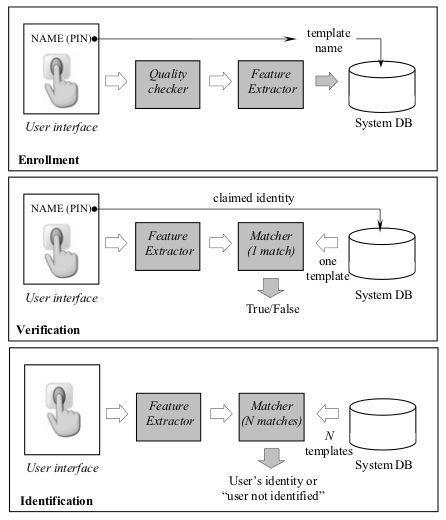
\includegraphics[scale=0.8]{three_way.png}
\caption{Schéma bloc de l'acquisition, de la vérification et de
  l'identification.}
\label{fig:schema-bloc-acq}
\end{figure}

Comme on peut le voir sur la Figure, l'image est ensuite transformée
en un modèle (\emph{template} en anglais) grâce à un extracteur de
caractéristiques (\emph{feature extractor} en anglais).

Dans le cas de la vérification, l'utilisateur entre son identifiant et
donne son empreinte. Celle-ci est transformée en un modèle compact.
On extrait le modèle lui correspondant dans la base de donnée, et un
comparateur est chargé de prendre la décision \og oui / non \fg.

Dans le cas de l'identification, c'est différent car il n'y a aucun
identifiant qui est donné et ce n'est plus un simple écart entre deux
modèles à calculer, mais un écart avec toutes les données de la base.
Les résultats possibles sont l'identité du possesseur des empreintes,
ou \og utilisateur non identifié \fg.

Il y a différentes parties distinctes, et dans un premier temps, nous
allons traiter des problèmes liés à ce type de biométrie. Dans un
second temps, nous allons traiter deux méthodes permettant la
vérification ou l'identification d'individu. La première de ces
méthodes et la méthode basé sur la corrélation entre deux empreintes
digitales. La seconde méthode se base sur les défauts que peuvent
présenter les empreintes digitales.


%%% Local Variables:
%%% mode: latex
%%% TeX-master: "../mlea"
%%% End:


\section{Problèmes liés à la biométrie}

Il y a divers problèmes liés à cette biométrie, notamment lors de
l'acquisition. Il y a principalement deux moyens d'effectuer ce
processus \emph{off-line}, c'est à dire la méthode ancestrale avec de
l'encre sur le doigt et apposé sur du papier, et \emph{live} qui
correspond à utiliser un scanner numérique. Pour assurer une
compatibilité entre ses deux méthodes d'acquisition, le ``US Criminal
Justice Information Services'' a présenté un ensemble de
spécifications pour fixer la qualité et le format des images (voir
annexes F et G de \cite{nla.cat-vn4185009}).

Bien que la méthode à l'encre ait commencé à être utilisé il y a très
longtemps (plus d'une trentaine d'année) elle est toujours utilisée
dans des applications à caractères légales. Les bases de données des
agences américaines de sécurités contiennent des données ayant été
acquises par les deux méthodes, ce qui signifie que les algorithmes
travaillant sur ces bases doivent être capables de les traiter
indépendemment.

Un des avantages d'utiliser l'acquisition avec l'encre est que l'on
peut enregistrer tout le doigt en effectuant un mouvement rotatif en
partant avec son doigt perpendiculaire d'un côté pour aller à
perpendiculaire de l'autre, ce qui n'est pas possible avec un scanner
numérique.

En contrepartie, il est possible, en fonction de comment est placée
l'encre sur le doigt, de laisser des zones de vide ou alors trop
pleine.

Du côté des acquisitions numériques, la plupart des appareils peuvent
se classer dans trois catégories différentes :

\begin{description}
\item[Optiques] le plus vieux et le plus utilisé des techniques
  d'acquisitions actuelles. Cette méthode fonctionne avec un prisme en
  verre. L'utilisateur doit mettre son doigt en haut de ce prisme est
  l'acquisition se fait ainsi.

  Ce type d'appareil a l'avantage de faire des images de bonnes
  qualités et d'avoir une grande surface du doigt enregistrée. Par
  contre, on ne peut pas miniaturiser cet appareil ;
\item[Ultrasons] il s'agit d'envoyer des ultrasons sur le doigt et de
  récupérer l'écho. Il est ainsi possible de dessiner la structure de
  l'empreinte digitale. Les images sont de bonne qualités, mais le
  système est onéreux ;
\item[Semi conducteurs] il y a quatre principales méthodes :
  thermique, capacitive, par champs électrique et piezoélectrique.  Il
  s'agit de toucher une carte en silice où chaque pixel est un petit
  capteur.
\end{description}

À présent que nous avons présenté les différentes manières de faire
l'acquisition, il nous faut à présent introduire quelques problèmes
communs à toutes les acquisitions. Il existe des variations en
fonction de l'état du doigt au moment de l'acquisition. Si celui-ci
est sec ou humide, l'image finale est différente.

Il existe aussi des problèmes de translation, de rotation ainsi que
des problèmes d'élasticité du doigt.


%%% Local Variables:
%%% mode: latex
%%% TeX-master: "../mlea"
%%% End:


\chapter{Correlation-based}
\chapter{Minuatiae Based}

La seconde méthode que nous allons traiter dans cet état de l'art est
la méthode basé sur l'extraction des minutia (ou minutiaes) sur les
empreintes digitales. Chaque empreinte comporte un certain nombre de
défaut, appelés minutiaes. Ces défauts sont unique pour chaque
individue. Cependant, il important de remarque que l'on a une chance
sur dix milliards d'avoir des minutia qui peuvent être assez
ressemblant pour être confondues. Les minutia sont des défauts de
l'empreinte digitales qui sont définie dès la naissance et qui sont
inchangeable durant la vie entière de l'individu.

Pour effectuer cette technique, il nous faut d'abord extraire un
maximum de ces défauts pour que la méthode puisse fonctionner d'une
façon optimale. Dans la seconde partie nous traiterons la méthode
permettant de valider si deux empreintes appartient bien au même
individu (et également au même doigt.)

\section{Détection des Minutiae}

Les minutiaes sont classés en divers types selon leurs spécification
et leurs formes géométrique et la typologies des lignes des
empreintes. L'A.N.S.I. (pour American Natiional Standards Insitute)

\section{Comparaison des minutiae}

Dans cette étape, on considère en entré deux ensembles: $p =
\{x_{i}^{p}, y_{i}^{p}, \theta_{i}^{p}\}, i \in \llbracket 1, M
\rrbracket$ et $q = \{x_{j}^{q}, y_{j}^{q}, \theta_{j}^{q}\}, j \in
\llbracket 1, N \rrbracket$ qui représentent les minutiae extraites de
chacune des images à comparer. La comparaison entre les deux
empreintes digitales se ramène ainsi à compter le nombre de paires de
minutiae identiques dans les deux ensembles et à comparer cette valeur
à un certain seuil. Cette comparaison se fait en deux étapes:

\begin{enumerate}
\item Trouver un alignement optimal;
\item Calculer la similarité.
\end{enumerate}

Pour chacune des ces étapes il existe plusieurs méthodes. Celle
présentée ci-dessous est tirée du cours~\cite{finger.00.jain} et les
illustration sont celles présentes dedans.

\subsection{Alignement}

Le problème d'alignement entre deux ensembles de minutiae est
compliqué car on ne sait pas à l'avance la correspondance entre les
minutiae des deux ensembles. De plus à cause des déformations dues au
bruit ajouté par les capteurs lors de l'acquisition des empreintes, il
est impossible de trouver un alignement exact. De ce fait l'alignement
entre les deux ensembles se fait en appliquant des déformations à l'un
jusqu'à minimiser la distance entre les deux ensembles. Ces
déformations sont de deux types: translations et rotations.\\

Plus précisément, le repère pour l'alignement sont les crêtes
représentées par des signaux en 1-dimension. L'algorithme d'alignement
prend en entré deux ensembles de crêtes venant de chacune des images:
$R_p$ et $R_q$ et se déroule comme suit:

\begin{enumerate}
\item Prendre une paire de crêtes: $c \in R_p$ et $c' \in R_q$ et les
  comparer utilisant la formule:
$$S = \frac{\sum\limits_{i=0}^L c_i c'_i}{\sqrt{\sum\limits_{i=0}^{L} c_{i}^2 c_{i}^{'2} }}$$
Avec:
\begin{itemize}
\item $L$: la taille de la plus petite crête
\item $c_i$: la distance du point $i$ de la crête $c$ à l'axe des abscisse
\item $c'_i$: la distance du point $i$ de la crête $c'$ à l'axe des abscisse
\end{itemize}
\item Si $S > seuil$ alors l'alignement est terminé.
\item Sinon:
  \begin{itemize}
  \item Calculer le vecteurs de translation:
    $$\Spvek{\Delta x \\ \Delta y} =  \Spvek{x_p \\ y_p} - \Spvek{x_q \\ y_q}$$
  \item Puis le vecteur de rotation:
    $$\Delta \theta  = \frac{1}{L} \sum\limits_{i = 0}^L (\varphi_i - \psi_i)$$
    avec $\varphi_i$ et $\psi_i$ les angles radiaux entre le $i^{ème}$
    point et la minutia de référence.
  \item Enfin appliquer la transformation suivante sur la minutiae:
    $$\Spvek{x_i \\  y_i \\ \theta_i} = \Spvek{\Delta x \\ \Delta y \\ \Delta \theta} +
    \left (
      \begin{array}{ccc}
        cos \Delta \theta & sin \Delta \theta & 0\\
        sin \Delta \theta & -cos \Delta \theta & 0\\
        0 & 0 & 1
      \end{array}
    \right )
    \Spvek{x_i - x_p \\ y_i - y_p \\ \theta_i - \theta_p}$$
  \end{itemize}
\item Recommencer à l'étape 1 avec une nouvelle paire de crêtes.
\end{enumerate}

Une fois que cette étape d'alignement est finie, l'alignement entre
les deux images est optimale et le calcul de similarité peut être
effectué.

\subsection{Calcul de similarité}

Une méthode pour calculer la similarité entre deux ensemble de
minutiae consiste à les considérer comme des chaînes de caractères et
appliquer un algorithme de calcul de distance d'édition sur les deux
chaînes.\\

La conversion des ensembles de minutiae en chaînes de caractères se
fait de la manière suivante: les coordonnées sont converties en
coordonnées polaires en fonction d'une minutiae de référence
choisie. Puis concaténer le résultat pour chaque minutiae par ordre
croissant d'angle radial:
$$P_p = \{(r_{1}^p, e_{i}^p, \theta_{1}^p), \ldots, (r_{M}^p, e_{M}^p, \theta_{M}^p)\}$$
$$Q_p = \{(r_{1}^q, e_{i}^q, \theta_{1}^q), \ldots, (r_{N}^q, e_{N}^q, \theta_{N}^q)\}$$

où $P$ et $Q$ sont donc deux chaînes de caractères.\\

La distance d'édition se calcule en utilisant un algorithme similaire
à celui de Levenshtein utilisant la programmation dynamique pour
remplir la matrice $C$:

$$C(m,n) = \left \{
\begin{array}{ll}
  0 & \mbox{ si } m = 0 \land n = 0\\
  min \left \{
      \begin{array}{l}
        C(m - 1, n) + \Omega\\
        C(m, n - 1) + \Omega\\
        C(m - 1, n - 1) + w(m, n)
      \end{array}  \right . & \mbox {sinon } 
\end{array} \right .
$$

Avec:

\begin{itemize}
\item $m \in \llbracket 0, M \rrbracket$ et $n \in \llbracket 0, N \rrbracket$
\item $w(m,n) = \left \{
    \begin{array}{ll}
      \alpha \mid r_{m}^p - r_{n}^q \mid + \beta \Delta e + \gamma \Delta \theta & \mbox { si } \mid r_{m}^p - r_{n}^q \mid < \delta \land \Delta e < \epsilon \land \Delta \theta < \rho \\
      \Omega & \mbox{ sinon}
    \end{array} \right .$
\item $\Delta e = \left \{
    \begin{array}{ll}
      a & \mbox { si } (a = (e_{m}^p - e_{n}^q + 360) \mbox{ mod } 360) < 180\\
      a - 180 & \mbox { sinon }
    \end{array} \right . $
\item $\Delta \theta = \left \{
    \begin{array}{ll}
      a & \mbox { si } (a = (\theta_{m}^p - \theta_{n}^q + 360) \mbox{ mod } 360) < 180\\
      a - 180 & \mbox { sinon }
    \end{array} \right . $
\end{itemize}

Et la signification des constante est la suivante:
\begin{itemize}
\item $\alpha$, $\beta$, $\gamma$ sont les poids associés au rayon,
  angle radial et orientation;
\item $\delta$, $\epsilon$, $\rho$ représentent la bounding-box;
\item $\Omega$ est une pénalité de différence fixé.
\end{itemize}

L'image~\ref{fig:match} présente un exemple graphique des résultats de
la méthode présenté.

\begin{figure}
  \centering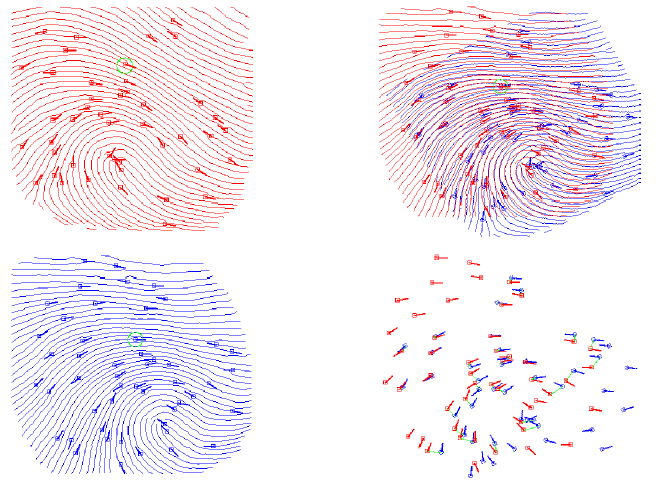
\includegraphics[scale=.4]{figres.png}
  \caption{Un exemple d'utilisation de la méthode.}
  \label{fig:match}
\end{figure}

La distance d'édition ainsi calculée est appelée $M_{pq}$ et permet de
calculer le score de similarité $S$ via la formule:
$$S = \frac{100 (M_{pq})^2}{MN}$$

La présentation donnée de l'algorithme possède quelque limitations, en
effet il tolère bien des transformations inexactes et/ou non linéaires
mais ne peut pas les compenser. Pour cela il faudrait utiliser la
méthode des bounding-box adaptative permettant une meilleur
correspondance entre les bounding box.\\

La complexité de l'algorithme de Levenshtein est avec l'implémentation
classique en $O(NM)$ avec $N$ et $M$ les tailles des deux
chaînes. Cependant un fort surcoût apparaît à cause du calcul des
différents poids et notamment de w. L'image~\ref{fig:recap} présente un schéma
récapitulatif de la méthode.

\begin{figure}
  \hspace{-10em}
  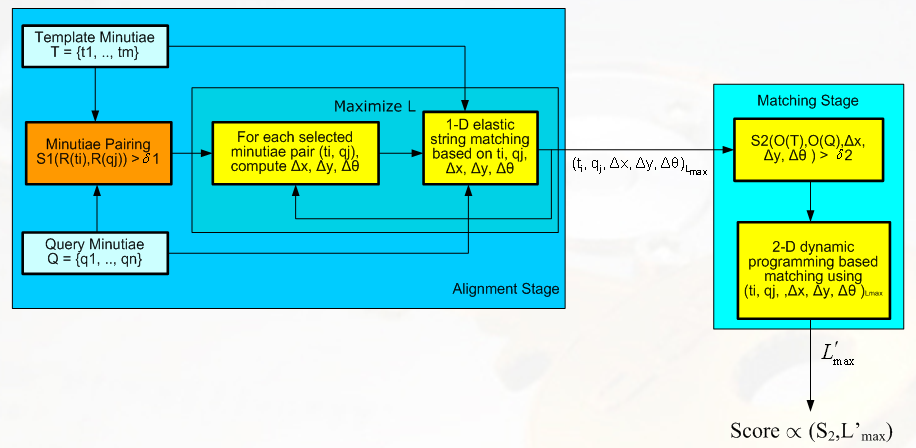
\includegraphics[scale=.6]{figrecap.png}
  \caption{Graphique récapitulant les grandes étapes de la méthode.}
  \label{fig:recap}
\end{figure}

\subsection{Performances}

En ce qui est des performance, cette méthode a été testé par les
auteurs de la présentation sur la base de données FVC2002 1. Cette
base contient 100 utilisateur avec chacun 8 empreintes.

Les résultats de la méthode sur cette base sont les suivants:
\begin{itemize}
\item Taux de fausses alarmes (FAR) : 0.1%
\item Taux de vrai acceptation (GAR) : 97.6%
\item Taux à erreurs égales (EER) : 1.65%
\item Taux de fausse acceptation (FRR) : 4%
\end{itemize}

De plus les courbes présentées dans l'image~\ref{fig:res} montrent
deux autres indicateurs. A titre de comparaison, l'algorithme donnant
les meilleur résultats sur cette base de donnée est PA15 et ses scores
sont les suivants:

\begin{itemize}
\item FAR : 0.11%
\item GAR : 100% 
\item EER : 0.1%
\item FRR : 0%
\end{itemize}

On se rend donc compte que cette méthode donne des résultats très
satisfaisant et est proche de la meilleur méthode. Un paramètre que
nous n'avons pas réussi à trouver est le temps que met la méthodes
pour donner un résultat donc nous ne pouvons pas comparer ce critère.

\begin{figure}
  \centering\subfloat[Distribution des similaritées]{\hspace{-10em}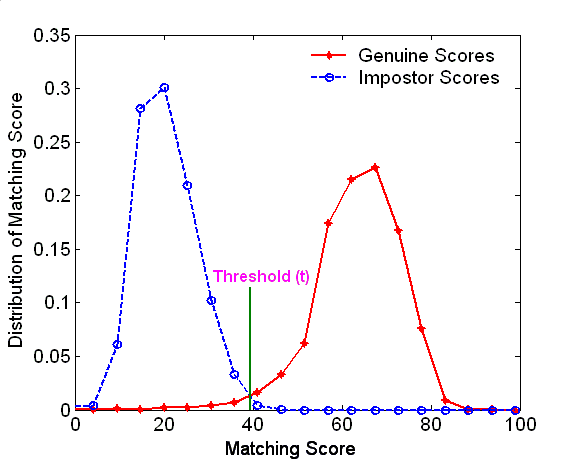
\includegraphics[scale=.5]{matchscore.png}}
  \centering\subfloat[Courbe ROC]{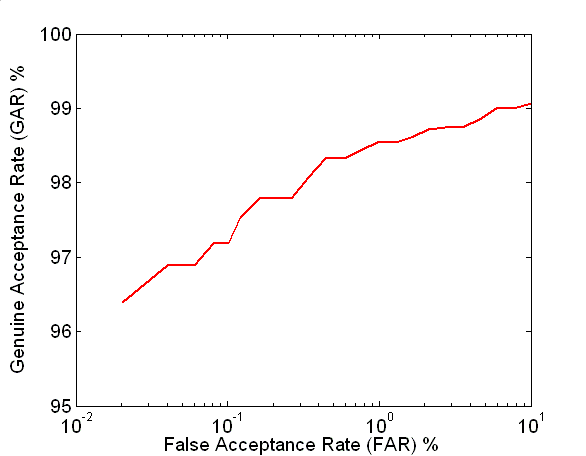
\includegraphics[scale=.5]{roccurve.png}}
  \caption{Deux autres indicateurs}
  \label{fig:res}
\end{figure}


\chapter{Conclusion}

\bibliography{mlea}

\end{document}



\bibliography{mlea}

\end{document}

%% mlea.tex end here

%  LocalWords:  American Institute
